\chapter{Introduction to Systems Programming in the Linux Computing Environment}
\section{Introduction}
\subsection{Objectives}
The purpose of this lab is to introduce system programming in a Linux development environment. After finishing this lab, students will be able to
\begin{itemize}
   \item use basic Linux commands to interact with the system through the shell
   \item use standard Linux C programming tools for system programming
   \item create a program to interact with the Linux file system using the relevant system and library calls.
\end{itemize}

\subsection{Topics}
Concretely, the lab will cover the following topics:
\begin{itemize}
  %\item how to connect to a remote Linux server;
  \item Basic Linux commands
  \item The C programming toolchain including \verb+gcc+, \verb+make+, and \verb+ddd+
  \item Linux manual pages
  \item Linux system calls and file I/O library calls and how to use them to traverse a directory and perform read/write operations on binary files
  \end{itemize}
  
\section{Starter Files}

The starter files are on GitHub at url: \url{http://github.com/broehl/ece252/}in the lab1/starter directory, which ontains the following sub-directories where we have example code and image files to help you get started:
\begin{itemize}
    \item \verb+cmd\_arg+ demonstrates how to capture command line input arguments
    \item \verb+ls+ demonstrates how to list all files under a directory and obtain file types
    \item \verb+png\_util+ provides a set of utility functions to process a PNG image file
    \item \verb+pointer+ demonstrates how to use pointers to access a C structure
    \item \verb+images+ contains some image files
    \item \verb+segfault+ contains a broken program that has a segmentation fault bug, which you will debug in the last pre-lab exercise.
\end{itemize}
Using the code in the starter files is permitted (and encouraged) and will not be considered as plagiarism.

\section{Pre-lab Preparation}

%Read Chapter \ref{ch_linux_env}. 
Read the Introduction to the ECE Linux Programming Environment supplementary material in Part \ref{part_ref} of this lab manual. Do the pre-lab exercises in Section \ref{sec_ex1}. Finish the pre-lab programming assignment before your scheduled lab starts (see \ref{sec:lab1_prelab_assignment}).
\subsection{Basic Linux Commands Exercises}
\label{sec_ex1}

These pre-lab exercises are to practice some basic commands on Linux. 
\begin{enumerate}
    \item Use MobaXterm to login onto
      \code{eceubuntu.uwaterloo.ca}. You are now inside the Linux shell and in your home directory. The home directory usually has a path name in the form \verb+/home/username+, where \code{username} is your UWID. For example, a user with UWID of \verb+jsmith+ has a home directory of \verb+/home/jsmith+.
    \item Use the \code{pwd} command to print the full pathname of the current working directory. You should see your home directory name printed on the screen. For example: \verb+/home/jsmith+.
    \item Use the \code{echo \$HOME} command to print your home directory path. You will notice that the output matches the \verb+pwd+ output of exercise 2.
    \item Use the \code{env} command to list all the environment variables and their values. Note that \verb+HOME+ is one of the many environment variables.
    \item One important environment variable is \verb+PATH+, which specifies a set of directories that the system searches for executable programs. Use \code{echo \$PATH} to see your \verb+PATH+ environment variable setting.
    \item Execute the command \code{which ls} to locate the directory the ls command is in. You will notice the directory is listed in the \verb+PATH+ environment variable. When you issue a command and get an error message of ``command not found'', it means the command cannot be found after searching all the directories listed in the \verb+PATH+ environment variable. A commonly seen error is that a command in your current working directory gives you a ``command not found`` error. This is normally due to the fact that the current working directory \verb+.+ or \verb+./+ is not in the PATH. Consequently you need to add the path to the command name for the system to know where the command is. For example \code{./a.out} tells the system to run the command \verb+a.out+ located in the current working directory. 
    \item Use the \code{ls} command to list all the files and directories in your current working directory. 
    \item Read the online manual of the \verb+ls+ command by issuing the
      \code{man ls} command to the shell.
      Find out from the manual what the options \verb+-l+, \verb+-a+ and \verb+-la+ do.
      Execute  the \verb+ls+ command with these three options and see the execution results.
    \item Create a directory called ECE252 under your home directory. You will use this for all your labs related to this course.
          Read the man page of the command \verb+mkdir+ to see how to do it.
    \item Change directory to the newly create directory of \verb+ECE252+.
          Read the man page of the command \verb+cd+ to find out how to change directory.
    \item Clone the ece252 lab repository by using the command: \\
      \code{git clone https://github.com/broehl/ece252.git}.

      A new directory named \verb+ece252+ will be created. It has the TeX source code for this lab manual and the starter code for each of the five labs. 
    \item Read the man page of the \verb+find+ command by issuing the
      \code{man find} command to the shell. Read what the \verb+-name+ option does. Use \verb+find+ with the \verb+-name+ option to find all the files with a ".png" file extension in the \verb+$HOME/ECE252/ece252+ directory.
    \item Change directory to where the file \verb+WEEF_1.png+ is. Use the command \code{file WEEF\_1.png} to obtain the file type and image properties such as dimensions and bit depth.
    \item Use the \verb+file+ command to obtain the file type information of \verb+Disguise.png+. You should see that this is not an image file, even though the file exension is .png.  Use a text editor to open the file and see the contents. This exercise is to show you that the \verb+file+ command does not obtain the file type information based on the file extension. It looks at the contents of that file to extract the file type information.
    \item You can use the command \verb+display+ to display an image. For example, to view the \verb+WEEF_1.png+ file, use the command \verb+display WEEF_1.png+. 
    \item Execute the \code{cat red-green-16x16.png} command and you will notice the output are gibberish. This is because cat is intended to display a plain text file, not a binary file. The PNG image file is a binary file. Both vi and emacs have a hexadecimal mode which displays the bytes in binary files in a hexadecimal format. They are pretty good for small size binary files. There are also few Linux commands that perform a hex dump of a file. One of them is called \verb+xxd+. Try \code{xxd red-green-16x16.png} and see the output. Other similar commands include \verb+od+ and \verb+hexdump+. Refer to the man pages of these commands for detailed usage instructions. 
    \item The \verb+pngcheck+ command tests PNG image files for corruption. Some image viewers are able to display an image even if part of it is corrupted. The fact that an image can be opened by an image viewer does not guarantee it is not corrupted. You will notice that the \verb+display+ command will not display a corrupted PNG image file on Linux. But the same corrupted image file most likely can be displayed by the Windows Paint program. Execute the following two commands and see what the pngcheck output tells you.
      \begin{itemize}
      \item \code{pngcheck red-green-16x16.png}
      \item \code{pngcheck red-green-16x16-corrupted.png}
      \end{itemize}
    \item Images are binary files. To compare two binary files, we can use the \verb+cmp+ command. Read the man page of the \verb+cmp+ command and especially pay attention to the \verb+-l+ option. Use the \verb+cmp+ command with the \verb+-l+ option to find out which bytes in \verb+red-green-16x16.png+ and \verb+red-green-16x16-corrupted.png+ are different. Another tool is \verb+vbindiff+, which displays and compares binary file(s).  
     \item Use gdb or ddd to run the program under in the lab1/starter/segfault directory of the starter code. When the code generates a segmentation fault inside the debugger, run the gdb command \code{where} to see the stack trace and fix the segmentation fault problem of the code. 
\end{enumerate}

\subsection{Pre-lab Assignment}
\label{sec:lab1_prelab_assignment}
You will write some small pieces of code that can be used in this and later lab assignments. You will create a command line program named \verb+pnginfo+ that prints the dimensions of a valid PNG image file or prints an error message if the input file is not a PNG file or is a corrupted PNG file. The command takes one input argument, which is the pathname of a file. Both absolute pathnames and relative path names are accepted. For example, if the input file is not a PNG file, the command \code{./pnginfo WEEF\_1.png} will output the following lines: 
\begin{verbatim}
WEEF_1.png: 450 x 229 
Disguise.png: Not a PNG file 
\end{verbatim}
If the input file is a PNG file, but some chunks have CRC errors (that is, the CRC value in the chunk does not match the CRC value computed by your program), then the program outputs something similar to what pngcheck does. For example, the command \code{./pnginfo red-green-16x16-corrupted.png} will output the following line:
\begin{verbatim}
red-green-16x16-corrupted.png: 16 x 16 
IDAT chunk CRC error: computed 34324f1e, expected dc5f7b84
\end{verbatim}

You will find the starter files in the png\_util directory are helpful. To make our pre-lab code reusable in the final lab, you should create two functions. One is \verb+is_png()+, which takes eight bytes and checks whether they match the PNG image file signature. The other function is \verb+get_data_IHDR()+, which extracts the image meta information including height and width from a PNG file IHDR chunk. You are free to design the signatures of these two functions so that they can be re-used in your lab1 final solution and future lab 2 and lab 3 solutions\footnote{lab2 and lab3 are based on the code of lab1}. However in \verb+lab_png.h+ you will find some existing function prototypes that we put there to show one possible function prototype design. Feel free to modify these function prototypes to fit your own design. For computing the CRC of a sequence of bytes, the starter code provides the files crc.c and crc.h along with a main.c file that demonstrates how to call the crc function to do the computation.
\section{Lab Assignment}
\subsection{Problem statement}

\begin{wrapfigure}{r}{2.5in}
  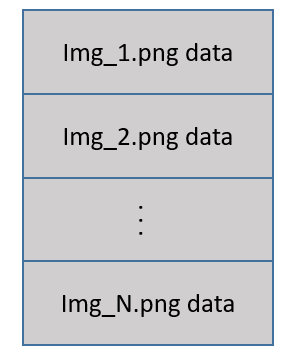
\includegraphics[width=2in]{img/img_concatenation}
  \caption{Image Concatenation Illustration}
\label{fig_img_concatenation}
\end{wrapfigure}

You are given a directory under which some files are PNG images and some files are not. The directory may contain nested sub-directories\footnote{A nested sub-directory is a sub-directory that may contain many layers of sub-directories.}. All valid PNG images under the given directory are horizontal strips of a bigger image. They all have the same width. The height of each image might be different. The PNG images have the naming convention of \verb+*_N.png+, where \verb+N+ is the image strip sequence number and \verb+N=0, 1, 2, ...+. However a file with a .png or .PNG extension may not be a real PNG image file. You need to locate all the real PNG image files under the given directory first. Then you will concatenate these horizontal image strips sequentially based on the sequence number in the file name to restore the original image. The sequence number indicates the position that the image should be placed in, from top to bottom. For example, the file \verb+img_1.png+ is the first horizontal strip and \verb+img_2.png+ is the second horizontal strip. To concatenate these two strips, the pixel data in the file \verb+img_1.png+ should be followed immediately by the pixel data in the file \verb+img_2.png+. Figure \ref{fig_img_concatenation} illustrates the concatenation order.

To solve the problem, first you will create a tool named \verb+findpng+ to search the given directory hierarchy to find all the real PNG files under it. Second, you will create an image data concatenation tool named \verb+catpng+ to concatenate the pixel data of a set of PNG files to form a single PNG image file. The \verb+catpng+ command only processes PNG images of the same width.
\subsection{The findpng command}
The expected behaviour of the \verb+findpng+ command is given in the following "manual page".
\subsubsection{Man page of findpng}
\subsubsection*{NAME}
\begin{itemize}
	\item[]{\bf findpng} - search for PNG files in a directory hierarchy
\end{itemize}
\subsubsection*{SYNOPSIS}
\begin{itemize}
	\item[]{\bf findpng} DIRECTORY 
\end{itemize}
\subsubsection*{DESCRIPTION}
\begin{itemize}
	\item[]Search for PNG files under the directory tree rooted at DIRECTORY and print the search results to the standard output. The command does not follow symbolic links.
\end{itemize}
\subsubsection*{OUTPUT FORMAT}
\begin{itemize}
	\item[]The output of search results is a list of relative pathnames\footnote{i.e. relative to the directory pathname on the command line} of the PNG files, one file pathname per line. The order of listing the search results is not specified. If the search result is empty, then output ``findpng: No PNG file found''.
\end{itemize}
\subsubsection*{EXAMPLES}
\begin{itemize}
	\item[]{\bf findpng .}
	\item[]Find PNG files under the current working directory. A non-empty search result might look like the following:
	\begin{verbatim}
	lab1/sandbox/new_bak.png
	lab1/sandbox/t1.png
	png_img/rgba_scanline.png
	png_img/v1.png
	\end{verbatim}
    It might also look like the following:
	\begin{verbatim}
	./lab1/sandbox/new_bak.png
	./lab1/sandbox/t1.png
	./png_img/rgba_scanline.png
	./png_img/v1.png
	\end{verbatim}
	An empty search result will look like the following:
	\begin{verbatim}
	findpng: No PNG file found
	\end{verbatim}
\end{itemize}
\subsubsection{Searching for PNG files under a given directory}
The Linux file system is organized as a tree. Every file has a type. Three file types that this assignment will deal with are regular files, directories and symbolic links.  A PNG file is a regular file. A directory is (unsurprisingly) a directory file. A link created by \verb+ln -s+ is a symbolic link. Read the description of the \code{stat} family of system calls in section 2 of the Linux man pages for information about other file types. The file \verb+ls/ls_ftype.c+ in the starter code gives a sample program to determine the type of a given file. Note that the \verb+struct dirent+ returned by the \verb+readdir()+ function has a field \verb+d_type+ that also gives the file type information. However, it is not supported by all file system types. We will be using our departmental Linux servers (eceubuntu) to test your submission. If you want to use the \verb+d_type+ field in your code, make sure you test its behaviour on the eceubuntu machines.

To search for all the files under a given directory and its subdirectories, you need to traverse the given directory tree to its leaf nodes.  The library call \code{opendir} returns a directory stream for \code{readdir} to read each entry in a directory. You need to call \code{closedir} to close the directory stream once operations on it are completed. The control flow is to go through each entry in a directory and check the file type. If it is a regular file, then further check whether it is a PNG file by comparing the first 8 bytes with the PNG file header bytes (see Section \ref{subsec_PNG_File_Format}). If it is a directory file, then you need to check files under the sub-directory and repeat what you did in the parent directory.
% The  \verb+chdir()+ family system calls change a working directory.
The file \verb+ls/ls_fname.c+ in the starter code contains a sample program that lists all the file entries of a given directory.
%The \verb+chdir/chdir1.c+ in the starter code gives one example of how to use the \verb+chdir()+ system call. 

Always check the man pages of the systems calls and library calls for detailed information.


\subsection{The catpng command}

The expected behaviour of the \verb+catpng+ command is given in the following "manual page".
\subsubsection{Man page of catpng}
\subsubsection*{NAME}
  \begin{itemize}
    \item[]{\bf catpng} - concatenate PNG images vertically to create a new PNG named "all.png"
  \end{itemize}
\subsubsection*{SYNOPSIS}
  \begin{itemize}
    \item[]{\bf catpng} [PNG\_FILE]... 
  \end{itemize}
\subsubsection*{DESCRIPTION}
  \begin{itemize}
  \item[]Concatenate PNG\_FILE(s) vertically to "all.png", a new PNG file.
  \end{itemize}
\subsubsection*{OUTPUT FORMAT}
  \begin{itemize}
  \item[]The concatenated image is output to  a new PNG file with the name of all.png.
  \end{itemize}
\subsubsection*{EXAMPLES}
\begin{itemize}
\item[]
\begin{verbatim}
catpng ./img1.png ./png/img2.png
\end{verbatim}
\item[]Concatenate the listed PNG images vertically to all.png.
\end{itemize}

\subsubsection{File I/O}
There are two sets of functions for file I/O operations under Linux. At the system call level, we have the {\em unbufferred I/O} functions: \code{open}, \code{read}, \code{write}, \code{lseek} and \code{close}. At the library call level, we have the standard I/O functions: \code{fopen}, \code{fread}, \code{fwrite}, \code{fseek} and \code{fclose}. The library is built on top of unbufferred I/O functions. It handles details such as buffer allocation and performing I/O in optimal sized chunks to minimize the number of \code{read} and \code{write} calls, so they're recommended for use in this lab.

The \code{fopen} function returns a FILE pointer given a file name and mode. A PNG image file is a binary file, hence when you call \code{fopen}, use mode "\code{rb}" for reading and "\code{wb+}" for reading and writing, where the "b" indicates it is a binary file that we are opening. Read the man page of \code{fopen} for more mode options. 

After the file is opened, use \code{fread} to read some number of bytes from the stream pointed to by the FILE pointer returned by \code{fopen}. Each opened file has an internal state that includes a file position indicator. The file position indicator is set to the beginning of the file when it is opened. The \code{fread} function will advance the file position indicator by the number of bytes that have been read from the file. The \code{fseek} function sets the file position indicator to the user-specified location. The \code{fwrite} function writes a user-specified number of bytes to the stream pointed to by the FILE pointer. The file position indicator also advances by the number of bytes that have been written. It is important to call \code{fclose} to close the file stream when I/O operations are finished. Failure to do so may result in incomplete files.  

The man pages of the standard I/O library are the main reference for details, including function prototypes and how to use them.   

\subsubsection{PNG File Format}
\label{subsec_PNG_File_Format}
In order to do this assignment, you need to have some understanding of the png file format and how an image is represented in the file. One way to store an image is to use an array of coloured dots referred to as {\em pixels}. A row of pixels within an image is called a {\em scanline}. Pixels are ordered from left-to-right within each scanline. Scanlines appear top-to-bottom in the pixel array. In this assignment, each pixel is represented as four 8-bit
\footnote{Formally, we say the image has a bit depth of 8 bits per sample.}
unsigned integers (ranging from 0 to 255) that specify the red, green, blue and alpha intensity values. This encoding is often referred to as the RGBA encoding. RGB values specify the colour and the alpha value specifies the opacity of the pixel. The size of each pixel is determined by the number of bits per pixel. The dimensions of an image are described in terms of horizontal and vertical pixels. 

% For each PNG pixel, there are five kinds of information namely read, green ,blue, greyscale, and alpha. A {\em channel} is an array of all per-pixel information of one of these five kinds. For example, the red channel is the array of red values of
\begin{figure}[h]  
\centering
\subfigure[PNG File Format] {
  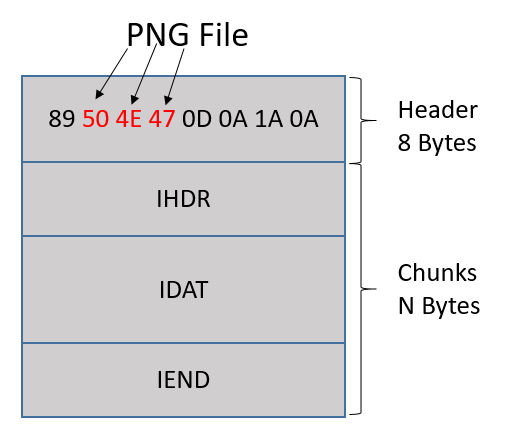
\includegraphics[width = 3in]{img/png_file_format}
  \label{fig_png_file_format}
}
\subfigure[PNG Chunk Format] {
  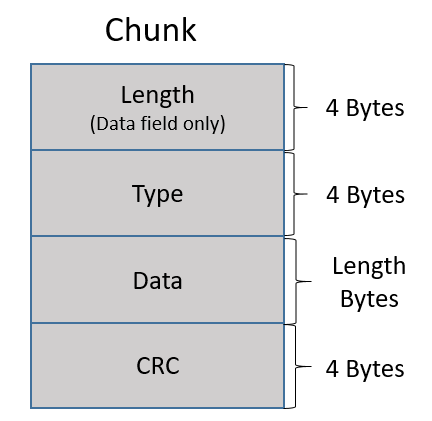
\includegraphics[width = 2.5in]{img/png_chunk_format}
  \label{fig_png_chunk_format}  
}
\end{figure}

PNG stands for ``Portable Network Graphics''. PNG is a file format for storing, transmitting and displaying images\cite{Roelofs1999PNG}. A PNG file is a binary file. It starts with an 8-byte header followed by a series of chunks. You will notice the second, third and fourth bytes are the ASCII codes for 'P', 'N' and 'G' respectively (see Figure \ref{fig_png_file_format}).

The first chunk is the IHDR chunk, which contains meta information about the image such as the dimensions in pixels. The last chunk is always the IEND chunk, which marks the end of the image data stream. In between there is at least one IDAT chunk which contains the compressed, filtered pixel array of the image. There are other types of chunks that may appear between the IHDR chunk and the IEND chunk. For all the PNG files we are dealing with in this assignment, there will only be on IHDR chunk, one IDAT chunk and one IEND chunk (see Figure \ref{fig_png_file_format}).


Each chunk consists of four parts. A four byte length field, a four byte chunk type code field, the chunk data field whose length is specified in the chunk length field, and a four byte CRC (Cyclic Redundancy Check) field (see Figure \ref{fig_png_chunk_format}).

The length field stores the length of the data field in bytes. PNG file uses {\em big endian} byte order, which is also the network byte order. When we process any PNG data that is more than one byte such as the length field, we need to convert the network byte order to host order before doing arithmetic. The \code{ntohl} and \code{htonl} library calls convert a 32 bit unsigned integer from network order to host order and vice versa respectively.



The chunk type code consists of four ASCII characters. IHDR, IDAT and IEND are the three chunk type codes that this assignment deals with.

The data field contains the data bytes appropriate to the chunk type. This field can be of zero length.

The CRC field stores a cyclic redundancy check on the preceding bytes in the type and data fields of the chunk. Note that the length field is not included in the CRC calculation. The \code{crc} function in the \verb+png_util+ starter code can be used to calculate the CRC value.

\begin{wraptable}{r}{3in}
	%\begin{table}
	\begin{center}
		\begin{tabular}{llc}             \toprule
			Name               & Length  & Value \\ \midrule
			Width              & 4 bytes & (varies)\\ \midrule
			Height             & 4 bytes & (varies)\\ \midrule
			Bit depth          & 1 byte  & 8\\ \midrule
			Colour type        & 1 byte  & 6\\ \midrule
			Compression method & 1 byte  & 0\\ \midrule
			Filter method      & 1 byte  & 0\\ \midrule
			Interlace method   & 1 byte  & 0\\ \bottomrule
		\end{tabular}
		\caption{IHDR data field and value}
		\label{lab1:tb_IHDR_Data}
	\end{center}
	%\end{table}
\end{wraptable}
The IHDR chunk data field has a fixed length of 13 bytes which appear in the order shown in Table \ref{lab1:tb_IHDR_Data}. Width and height are four-byte unsigned integers giving the image dimensions in pixels. You will need these two values to complete this assignment. Bit depth gives the number of bits per sample. In this assignment, all images have a bit depth of 8. Colour type defines the PNG image type. All png images in this assignment have a colour type of 6, which is truecolor with alpha (i.e. RGBA image). The image pixel array data is filtered to prepare for the next step of compression. The Compression method and Filter method bytes encode the methods used. Both only have 0 values defined in the current standard. The Interlace method indicates the transmission order of the image data. 0 (no interlace) and 1 (Adam7 interlace) are the only two defined. In this assignment, all PNG images are non-interlaced. The Value column in table \ref{lab1:tb_IHDR_Data} gives the typical IHDR values for the PNG images that you will be processing.  

The IDAT chunk data field contains compressed filtered pixel data. For each scanline, an extra byte is added at the very beginning of the pixel array to indicate the filter method used. Filtering is for preparing for the next step of compression. For example, if the raw pixel scanline is 4 bytes long, then the scanline after applying the filter will be 5 bytes long. This additional one byte per scanline will help to achieve better compression results. After all scanlines have been filtered, the data are compressed according to the compression method encoded in the IHDR chunk. The compressed data stream conforms to the zlib 1.0 format.

The IEND chunk marks the end of the PNG datastream. It has an empty data field.

\subsubsection{Concatenate the pixel data}
To concatenate two horizontal image strips, the natural approach would be to start with the pixel array for each image and then concatenate the two pixel arrays vertically. Then we would apply the filter to each scanline. Lastly we would compress the filtered pixel array to fill the data field of the new IDAT chunk of the concatenated image.

However, a simpler method exists. We can start with the filtered pixel data of each image and then concatenate the two chunks of filtered pixel data arrays vertically, then apply the compression method to generate the data field of the new IDAT chunk.

How do we get filtered pixel data from a PNG IDAT chunk? Recall that the data field in an IDAT chunk is compressed using zlib format 1.0. We can use zlib library functions to inflate (i.e. uncompress) the data. The \code{mem\_inf} function in the starter code takes in-memory deflatd (i.e. compressed) data as input and stores the uncompressed data in a given memory location. For each IDAT chunk you want to concatenate, you call this function and stack the returned data in the order you wish in order to obtain the concatenated filtered pixel array. To create an IDAT chunk, we need to compress the filtered pixel data. The \code{mem\_def} function in the starter code uses zlib to deflate (i.e. compress) the in-memory data and returns the deflated (i.e. uncompressed) data. The \verb+png_util+ directory in the starter code demonstrates how to use these two functions.

To create a new PNG file for the concatenated images, an IHDR chunk also needs to have the dimensions of the new PNG file. The rest of the fields of the IHDR chunk can be kept the same as one of the PNG files to be concatenated. In this assignment, we assume that \verb+catpng+ can only process PNG files whose IHDR chunks only differ in the height field. So the new image will have a different height field, andand  the rest of the fields are the same as the input images.



\section{Deliverables}
\subsection{Pre-lab deliverables}
\label{lab1_prelab_deliverable}
The pre-lab is due by the time that your scheduled lab sessions starts. No late submission of the pre-lab is accepted. Grace days are not applicable to pre-lab submissions. The following are the steps to create your pre-lab deliverable submission.
\begin{itemize}
\item Create a directory under your ECE252 directory and name it lab1-pre.
\item Put the entire source code with a Makefile under the directory lab1-pre. The Makefile default target includes \verb+pnginfo+. That is, the command \verb+make+ should generate an executable file of that name. We also expect that the command \verb+make clean+ will remove the object code and the default target. That is, the \verb+.o+ files and the executable file should be removed.
\item Use the \verb+zip+ command to zip up the contents of the lab1-pre directory and name it \verb+lab1-pre.zip+. We expect that \verb+unzip lab1-pre.zip+ will produce a \verb+lab1-pre+ sub-directory in the current working directory and under the \verb+lab1-pre+ sub-directory will be your source code and the Makefile.
\end{itemize}
Submit the \verb+lab1-pre.zip+ file to the Lab1 Pre-lab Dropbox on Learn by the time your scheduled lab session starts. The TA on duty will evaluate the pre-lab by letting you demo the submitted program during the scheduled lab session.

\subsection{Post-lab Deliverables}
The post-lab is due two days after your scheduled lab session at 22:00. Grace days can be used towards late submissions of the post-lab deliverable. The following are the steps to create your post-lab deliverable submission.
\begin{itemize}
\item Create a directory under your ECE252 directory and name it lab1.
\item Put the entire source code with a Makefile under the directory lab1. The Makefile default target includes \verb+catpng+ and \verb+findpng+. That is, the command \verb+make+ should generate these two executable files. We also expect that the command \verb+make clean+ will remove the object code and the executables. That is, the \verb+.o+ files and the two executable files should be removed.
\item Use the \verb+zip+ command to zip up the contents of the lab1 directory and name it lab1.zip. We expect \verb+unzip lab1.zip+ will produce a \verb+lab1+ sub-directory in the current working directory and under the \verb+lab1+ sub-directory will be your source code and the Makefile.
\end{itemize}
Submit the \verb+lab1.zip+ file to the Lab1 Dropbox on Learn.
\section{Marking Rubric}
\begin{table}[ht]
\begin{center}
\begin{tabular}{|p{2cm}|p{2cm}|p{9cm}|}
\hline
Points & Sub-points &Description  \\ \hline
15     &   & Pre-lab      \\ \hline
       & 2 & \verb+Makefile+ correctly builds and cleans \\ \hline
       & 13& Implementation of \verb+pnginfo+ \\ \hline
%       & 3 & \verb+ckpng+ detects a non-png file type \\ \hline
%       & 5 & \verb+ckpng+ prints non-corrupted png image dimensions \\ \hline
%       & 5 & \verb+ckpng+ detects incorrect CRC of the simple PNG data chunk \\ \hline
85     &        & Post-lab \\ \hline
       & 10     & Makefile correctly builds and cleans \\ \hline
       & 30     & Implementation of \verb+findpng+  \\ \hline
       & 45     & Implementation of \verb+catpng+ \\ \hline
\end{tabular}
\caption{Lab1 Marking Rubric}
\label{tb_lab1_rubric}
\end{center}
\end{table}

Table \ref{tb_lab1_rubric} shows the rubric for marking the lab. Note that if your code generates a segmentation fault, the maximum lab grade you can achieve is 60/100.

%%% Local Variables:
%%% mode: latex
%%% TeX-master: "main_book"
%%% End:
